\documentclass[12pt]{article}
\usepackage{amsfonts}
\usepackage{amsmath}
\usepackage{graphicx} 
\usepackage{float}
\usepackage{xcolor}
\usepackage[caption = false]{subfig}
\usepackage[
backend=biber,
style=authoryear,
maxcitenames=3,
maxbibnames=3,
uniquelist=false,
backref=true,
doi=false,
isbn=false,
url=false,
eprint=false,
backref=false
]{biblatex}
\addbibresource{/Users/timbarry/optionFiles/tims_proposal.bib}
\usepackage{/Users/timbarry/Documents/optionFiles/mymacros}

\begin{document}
	\noindent
	Tim B.
	\begin{center}
		\textbf{The overlooked need for negative controls in conditional independence testing}
	\end{center}

\section{Introduction}

Conditional independence (CI) tests asses the association between two variables (e.g., a genetic variant and a phenotype) while controlling for a vector of confounders (e.g., population structure). CI tests are among the most fundamental and widely-used hypothesis tests in the sciences, technology, and other areas. Despite their importance, CI tests pose a basic and unavoidable difficulty: assumption-free CI testing is impossible \parencite{Shah2020,Kim2021}. Put differently, all valid CI tests must make an assumption (or set of assumptions) about the data-generating process. In practice these assumptions are seldom checked, greatly limiting the trustworthiness of results. This is not due to negligence; to the contrary, checking the assumptions of CI tests is fraught with difficulties, as we will show. We therefore face a dilemma as data analysts: we are obligated to check the assumptions of CI testing procedures to ensure reliableness of the results, but very often this is challenging (or impossible) to do.

Our core thesis is that ``negative controls'' -- external samples for which the null hypothesis is known to be true, roughly  -- are crucially important (and in some cases \textit{required}) for verifying the assumptions of CI testing procedures, enabling rigorous inference. We work in the contemporary ``high-multiplicity'' setting in which we seek to test thousands (or more) of hypotheses and produce a discovery set with guaranteed false discovery rate (FDR) control \parencite{Benjamini1995, Li2021}.

First, we briefly summarize the vast and growing landscape of CI testing procedures, omitting from our discussion those procedures that do not enable the selection of critical regions (and thus the control of FDR). We argue that negative controls play (or ought to play) a crucial role in high-multiplicity CI testing. We describe two broad types of negative controls --- ``experimental'' negative controls and ``in silico'' negative controls --- and argue that, although the former are superior statistically, the latter can be constructed directly from the data in many applications and are therefore more broadly available.

Next, we introduce several new strategies for working effectively with negative control data in high-multiplicity hypothesis testing problems. (The discussion here extends beyond CI testing.) We propose to calibrate the testing procedure against \textit{both} the empirical negative control distribution \textit{and} the theoretical null distribution, satisfying an appealing double-robustness property. We also introduce a simple and practical method for assessing whether a given procedure is robust to inflation (or deflation) in the tail of the empirical null distribution. Finally, we introduce the ``symmetry plot'' (or ``s-plot''), a nonparametric analogue of the commonly-used quantile-quantile plot (qq-plot) to aid in the application of the above methods. % Throughout, we lean heavily on the Barber-Candes (BC) multiple testing procedure \parencite{Barber2015}, as we find this approach to be flexible, extensible, and powerful. 

As an auxiliary contribution, we introduce a new class of fast and powerful Gaussian test statistics for use in a broad range of existing CI testing methods, including the conditional randomization test, the conditional permutation test, and the local permutation test \parencite{Candes2018a,Berrett2020,Kim2021}. The idea behind these statistics is to repeatedly fit OLS, ridge regression, or additive spline models to the permuted (or resampled) data via an online QR decomposition, achieving high speed and power. % These statistics also are compatible with standard permutation tests of (marginal) independence.
We apply the ideas that we introduce to analyze a new and important type of biological data that combines CRISPR genome editing with single-cell RNA sequencing.

\section{A brief taxonomy of CI testing methods}

There exist myriad methods for testing CI; see \cite{Kim2021} for a recent review. Inspired by \cite{Kim2021}, we consider a simplified ``taxonomy'' of CI testing methods that consists of four categories: (i) standard parametric, (ii) model-X, (iii) matching, and (iv) nonparametric asymptotic. The first two categories are model-based (in that they assume a model --- possibly up to a parametric family --- for the data generating process), and the latter two are model-free. Figure \ref{cimethods} illustrates these categories and provides an example of each.

We briefly review CI testing methods that fall into these categories and highlight their underlying assumptions. Standard parametric approaches assume that the distribution $\mathcal{L}(Y|X,Z)$ of $Y$ given $X$ and $Z$ is known up to parametric family; examples include GLMs. Inference (typically) is based on the CLT, which, in addition to correct model specification, requires the number of samples to be large relative to the number of parameters. Model-X approaches make the rather strong (and sometimes reasonable) assumption that the distribution $\mathcal{L}(X|Z)$ of $X$ given $Z$ is known exactly. An example is the conditional randomization test (CRT; \textcite{Candes2018a}). Inference in model-X methods is exact in finite samples.

Matching-based approaches test for CI by grouping observations based on their vector of confounders $Z$. An example is the recently-proposed local permutation test (LPT; \textcite{Kim2021}). The LPT approximates the joint distribution $(Y, X, Z)$ by $(Y, X, \tilde{Z}),$ where $\tilde{Z}$ is a discretized version of $Z$. The LPT assumes that $X \indep Y | \tilde{Z}$ implies $X \indep Y | Z$ and uses a permutation-based approach to test the former hypothesis. Finally, the nonparametric asymptotic approach leverages nonparametric regression and/or density estimators to construct a test statistic whose asymptotic distribution is known under the null hypothesis. An example is the generalized covariance measure (GCM; \textcite{Shah2020}). GCM estimates the regression functions $f(z) := \E[X|Z = z]$ and $g(z) := \E[Y|Z = z]$ using (possibly black box) regression estimators and constructs an asymptotically Gaussian test statistic by taking a normalized product of the residuals. GCM assumes that the regression functions $f$ and $g$ can be estimated sufficiently fast.

We emphasize that each of the above approaches makes an assumption or set of assumptions about the joint distribution $\mathcal{L}(X,Y,Z)$. These assumptions are mathematically concrete and could in theory be checked by an oracle with knowledge of the joint distribution. In practice, of course, we do not have knowledge of $(X,Y,Z)$ and thus must consider other strategies for assumption checking.

\begin{figure}
	\centering
	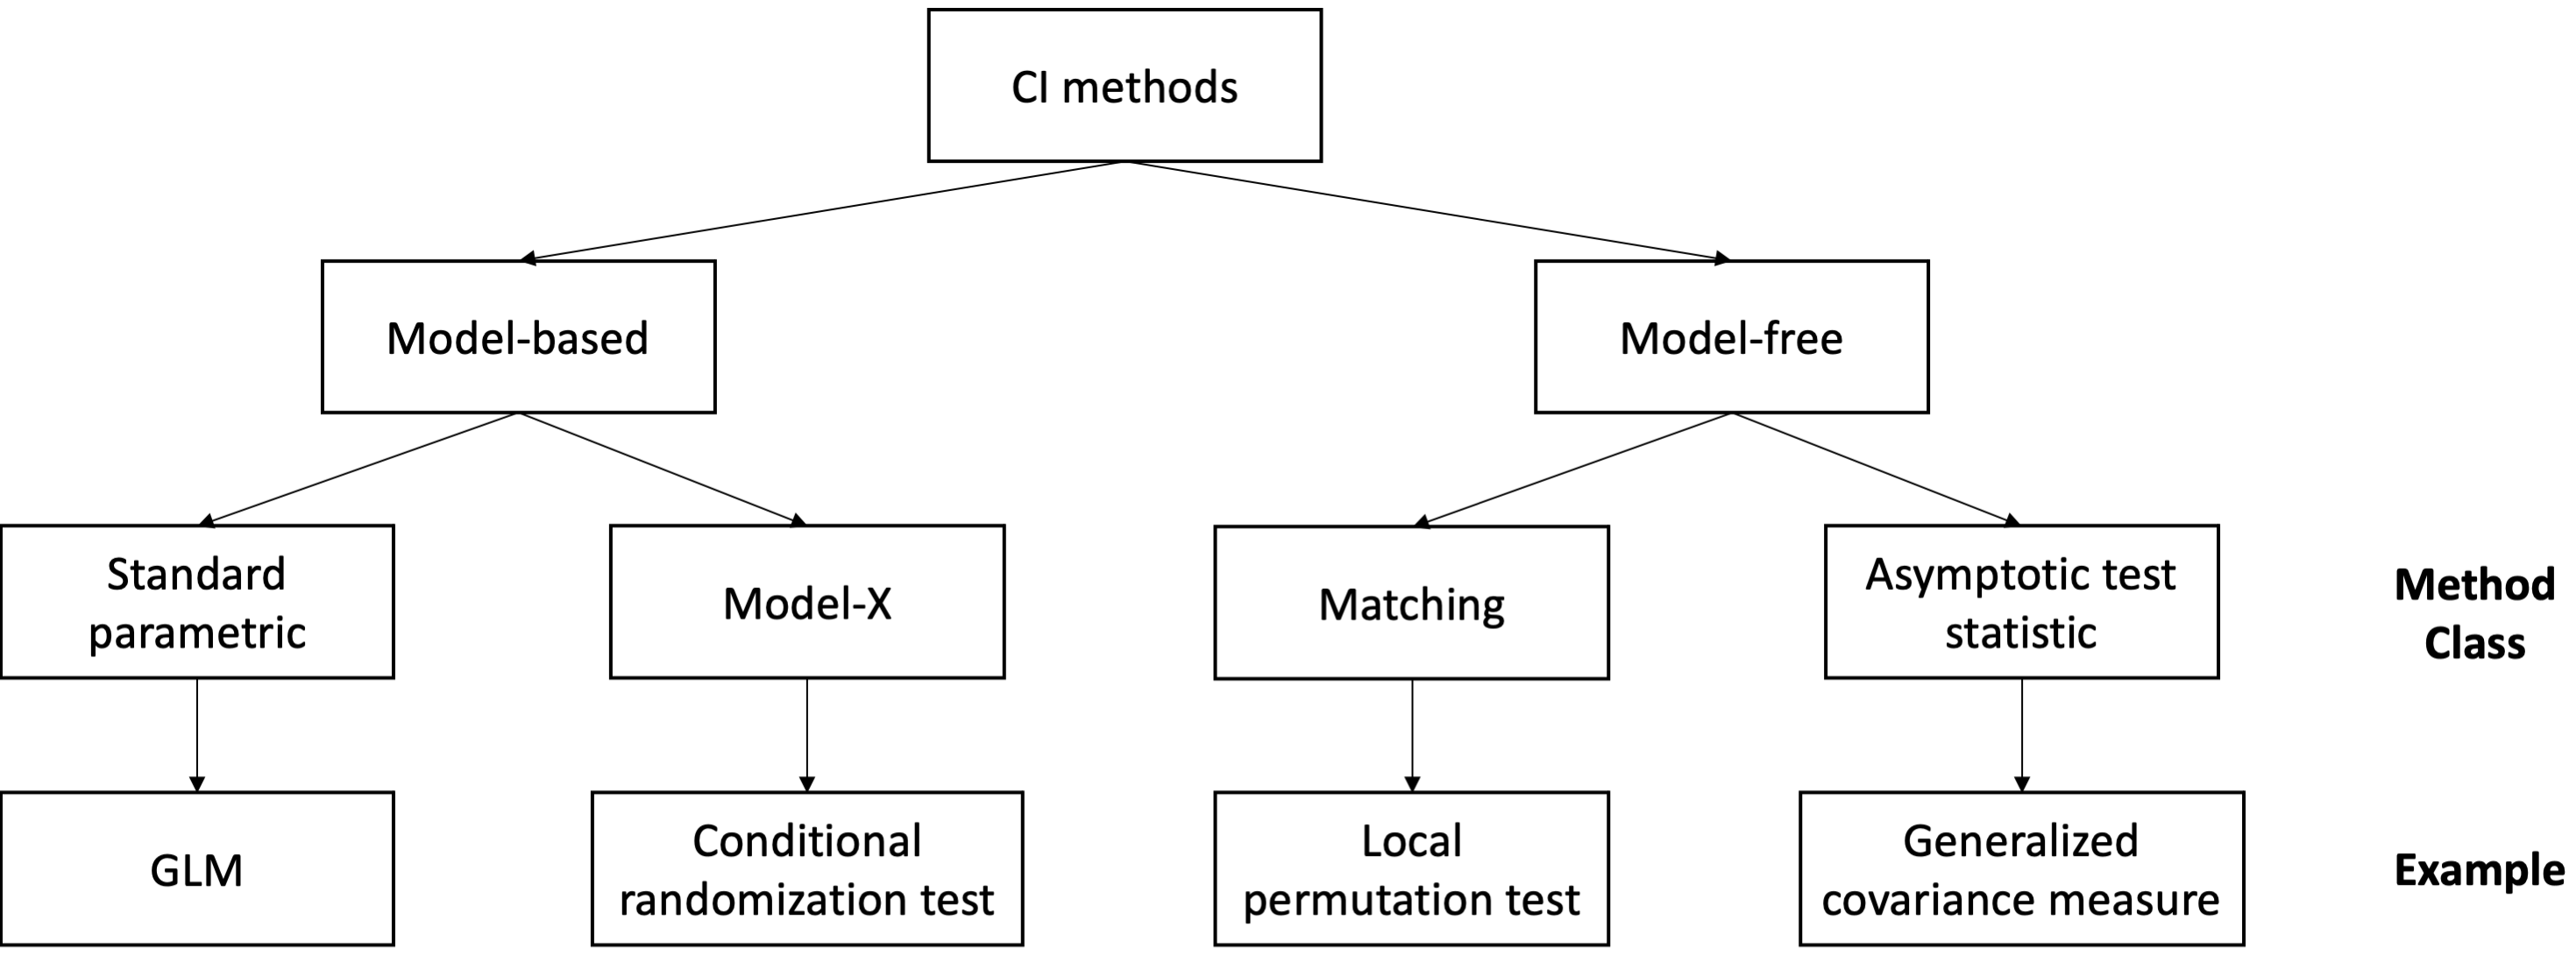
\includegraphics[width=1\linewidth]{../figs/CI_methods}
	\caption{An abbreviated taxonomy of CI testing methods.}
	\label{cimethods}
\end{figure}

\section{The crucial importance --- and difficulty --- of assumption checking in CI testing}

Assumption checking is of crucial importance in CI testing. Consider the local permutation test (LPT) of \cite{Kim2021} as an illustrative example. \textcolor{blue}{[Insert a small simulation study applying LPT to synthetic data for which the assumptions of LPT are violated. Show that, in the absence of assumption checking, type-I error inflation and FDR violation can be severe.]}

Unfortunately, the assumptions underlying LPT are uncheckable (absent additional, external information). Let $P^n_{X,Y,Z}$ denote the product distribution of the observed data $(X_1, Y_1, Z_1), \dots, (X_n, Y_n, Z_n)$. Next, let $Q^n_{X, Y, \tilde{Z}}$ denote the distribution that results from discretizing $Z$. Finally, let $\tilde{Q}^n_{X,Y,\tilde{Z}}$ denote the closest distribution (in TV distance) to $Q^n_{X,Y,\tilde{Z}}$ in the space of distributions for which $X \indep Y | \tilde{Z}.$ \textcite{Kim2021} show that the excess type-I error of LPT is bounded above by $d_{\textrm{TV}}\left( \tilde{Q}^n_{X,Y,\tilde{Z}}, \tilde{Q}^n_{X,Y,\tilde{Z}} \right)$. They furthermore derive an explicit, analytic upper bound that holds if the conditional distributions $\mathcal{L}(X|Z=z)$ and $\mathcal{L}(Y|Z=z)$ are sufficiently smooth as $z$ varies. Although theoretically informative, these bounds cannot be evaluated in practice, as the densities $\mathcal{L}(X,Y,Z),$ $\mathcal{L}(X|Z)$, and $\mathcal{L}(Y|Z)$ are unknown. We highlight LPT only to provide the reader with a concrete example; other model-free approaches (e.g., GCM) likewise place assumptions on $\mathcal{L}(X,Y,Z)$ that cannot be checked in practice.

Assumption checking in model-based approaches likewise is fraught with challenges, especially in high dimensions. Suppose that we test CI by fitting a linear model to the data. Goodness-of-fit checks that work well in low dimensions --- e.g., calculating likelihood-based metrics such as AIC, estimating predictive performance via cross-validation, etc. --- break down in high-dimensions. For example, overfitting can render meaningless metrics based on likelihood, and predictive performance does not necessarily provide much information about estimation performance. (In fact, prediction and estimation risk are inversely related in the high-dimensional linear model; \textcite{Dobriban2018}.) Therefore, model-based approaches pose similar challenges with respect to model checking to model-free approaches, especially in high-dimensions. \textcolor{blue}{[Can we prove a general result about the impossibility of checking assumptions of CI tests?]}

\section{The need for negative controls} 

We make two distinctions. First, we distinguish between ``calibration data'' and ``test data.'' Calibration data are negative control data on which we assess calibration, and test data are data on which apply our procedure with the objective of obtaining FDR control. Ideally, the calibration and test data are different, but in some applications they may coincide. 

\begin{itemize}
	\item single-cell CRISPR screens
	\begin{itemize}
	\item Experimental controls typically are available.
	\item When they are not, pair perturbations to genes on different chromosomes, avoiding transcription factors.
	\end{itemize}
	\item eQTLs
	\begin{itemize}
	\item Pair SNPs to genes on different chromosomes, again avoiding transcription factors.
	\end{itemize}
	\item multimodal single-cell data (e.g., chromatin accessibility and gene expression)
	\begin{itemize}
	\item Pair chromatin regions with genes on other chromosomes, again avoiding transcription factors.
	\end{itemize}
	\item bulk RNA-seq
	\begin{itemize}
	\item Really, we are testing a conditional independence hypothesis here: is there differential expression \textit{conditional} on the library size? Most genes are not differentially expressed, and so they can serve as negative controls. Here, calibration and test data coincide.
	\end{itemize}
\end{itemize}

% NCs likewise require us to make an assumption (roughly, that the negative controls carry some information about the test data). 
\section{Strategies for working effectively with negative controls}

We hope that the reader is convinced that (i) negative controls are of crucial importance in conditional independence testing and that (ii) negative controls --- either experimental or \textit{in silico} --- are available or can be constructed for many important datasets, especially those in genomics and genetics. A natural question, then, is ``How can we work effectively with negative control data?'' We take steps toward answering this question. We propose to calibrate the test procedure against \textit{both} the empirical negative control distribution \textit{and} the theoretical null distribution, satisfying a double-robustness property. First, we take a slight detour to introduce ``symmetry plots,'' nonparametric analogues of qq-plots.

\subsection{Symmetry plots (s-plots)}

Symmetry plots (``s-plots'') are visual diagnostics that track the extent to which an empirical distribution is symmetric about zero. Let $X_1, \dots, X_B \sim F$ be samples from some common distribution with density function $f$. Assume that $B$ is even (otherwise, throw out the median). Let $X_{(1)}, \dots, X_{(B)}$ be the order statistics of $X_1, \dots, X_B$. Consider the set
$$ \mathcal{S} := \{(-X_{(1)}, X_{(B)}), \dots, (-X_{(i)}, X_{(B - i +1)}), \dots, (-X_{(B/2)}, X_{(B/2 + 1)})\},$$ i.e., pair the negative of the first order statistic with the last order statistic, the negative of the second order statistic with the penultimate order statistic, etc. An s-plot is a plot of the set $\mathcal{S}.$ If the underlying density function $f$ is symmetric about zero, then the points fall approximately onto the identity line $y=x$. Figure \ref{splot} shows a histogram, s-plot, and qq-plot of $B=10,000$ draws from a double-exponential distribution. Clearly, the histogram (left) is not Gaussian (blue curve indicates Gaussian MLE); accordingly, the qq-plot (right) exhibits inflation in the tail. However, the double-exponential distribution is symmetric about zero; hence, the s-plot closely follows the identity line. 

The rationale for the s-plot is as follows. The expected value of $X_{(i)}$ should be a quantile of order $(i - 1/2)/B$. Meanwhile, the expected value of $X_{(B-i+1)}$ should be a quantile of order $[B - i + 1/2]/B.$ Note that $$[i - 1/2]/B + [B - i + 1/2]/B = 1.$$ Because $f$ is symmetric about the origin, it follows that
$$-F^{-1}([i-1/2]/B ) = F^{-1}([B-i+1/2]/B).$$
Thus,
$$\E[-X_{(i)}] \approx -F^{-1}([i - 1/2]/B) = F^{-1}([B - i + 1/2]/B) \approx \E[X_{(B-i+1)}],$$ implying the points in the s-plot lie approximately along the identity line.
% \textcolor{blue}{[It would be good to good pointwise confidence intervals for s-plots.]}
\begin{figure}
	\centering
	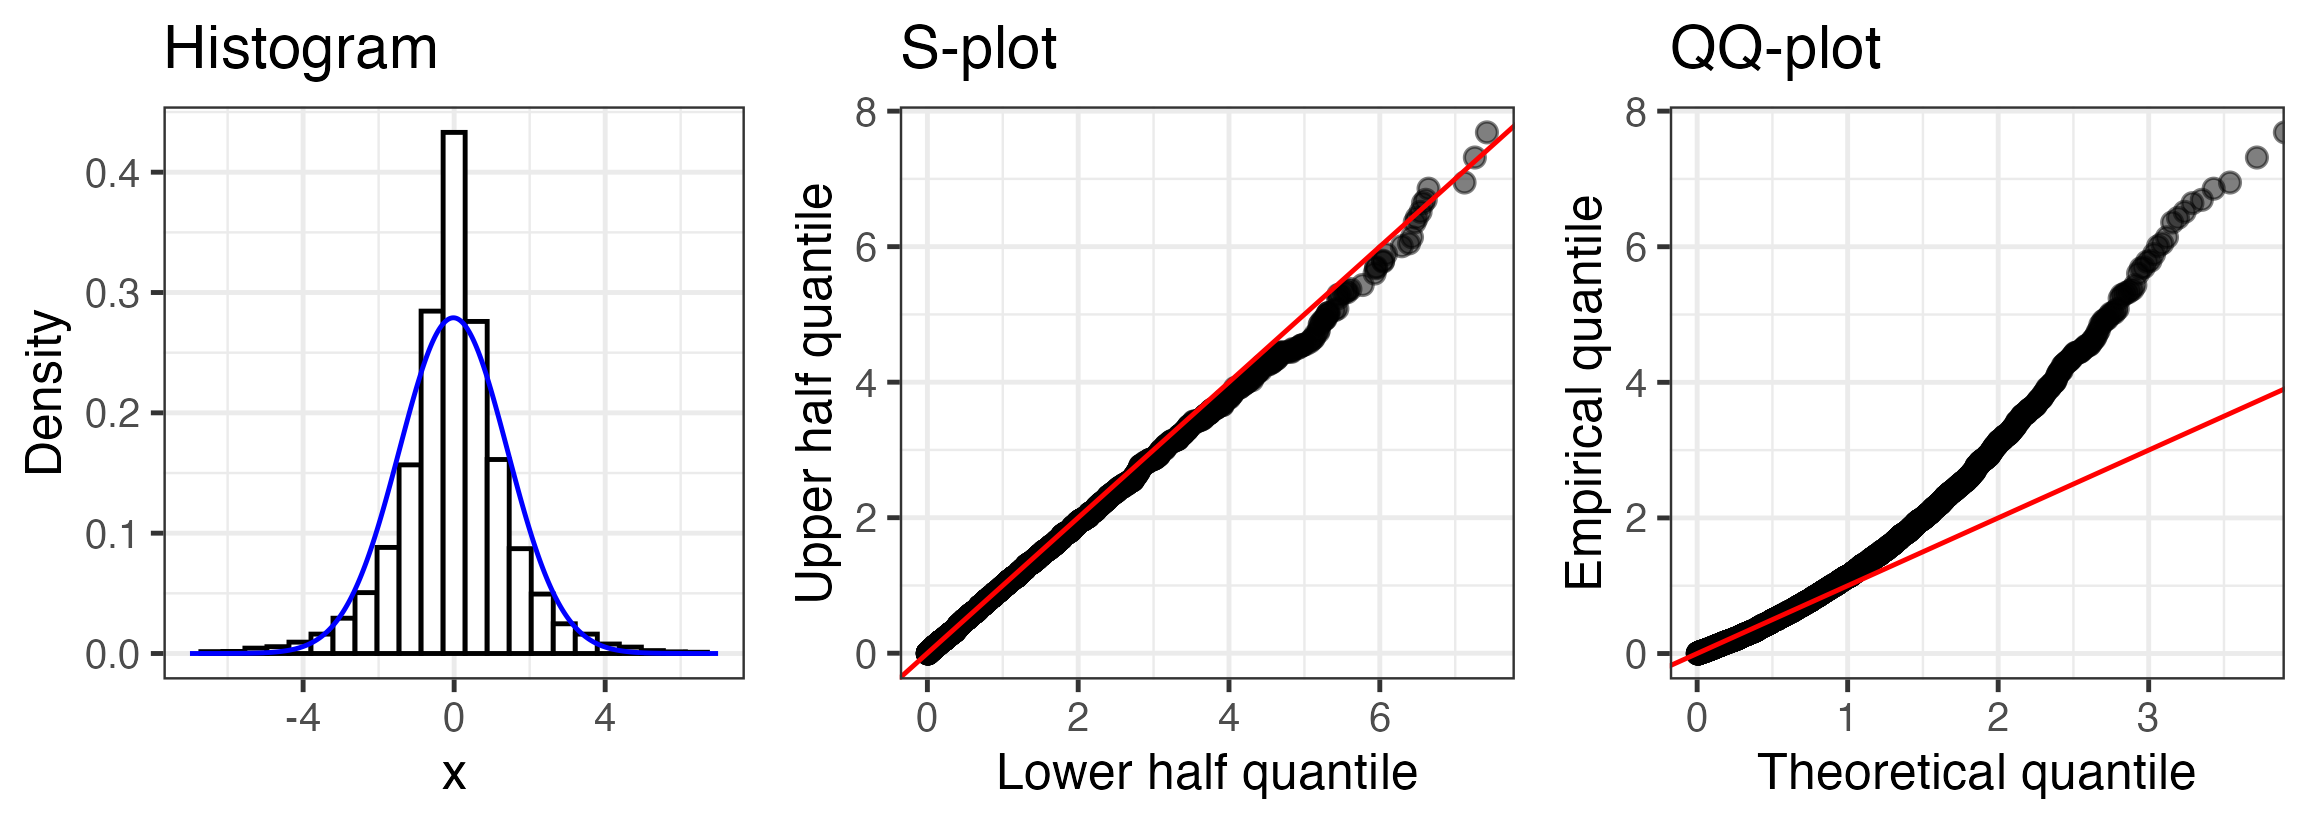
\includegraphics[width=1.0\linewidth]{../figs/s_plot}
	\caption{Histogram, s-plot, and qq-plot (only right tail shown) of $B=10,000$ draws from a double-exponential distribution.}
	\label{splot}
\end{figure}

\subsection{The Barber-Cand\'es method and symmetry-preserving transformations}

The Barber-Cand\'es method is a flexible method for FDR control. 

\begin{figure}
	\centering
	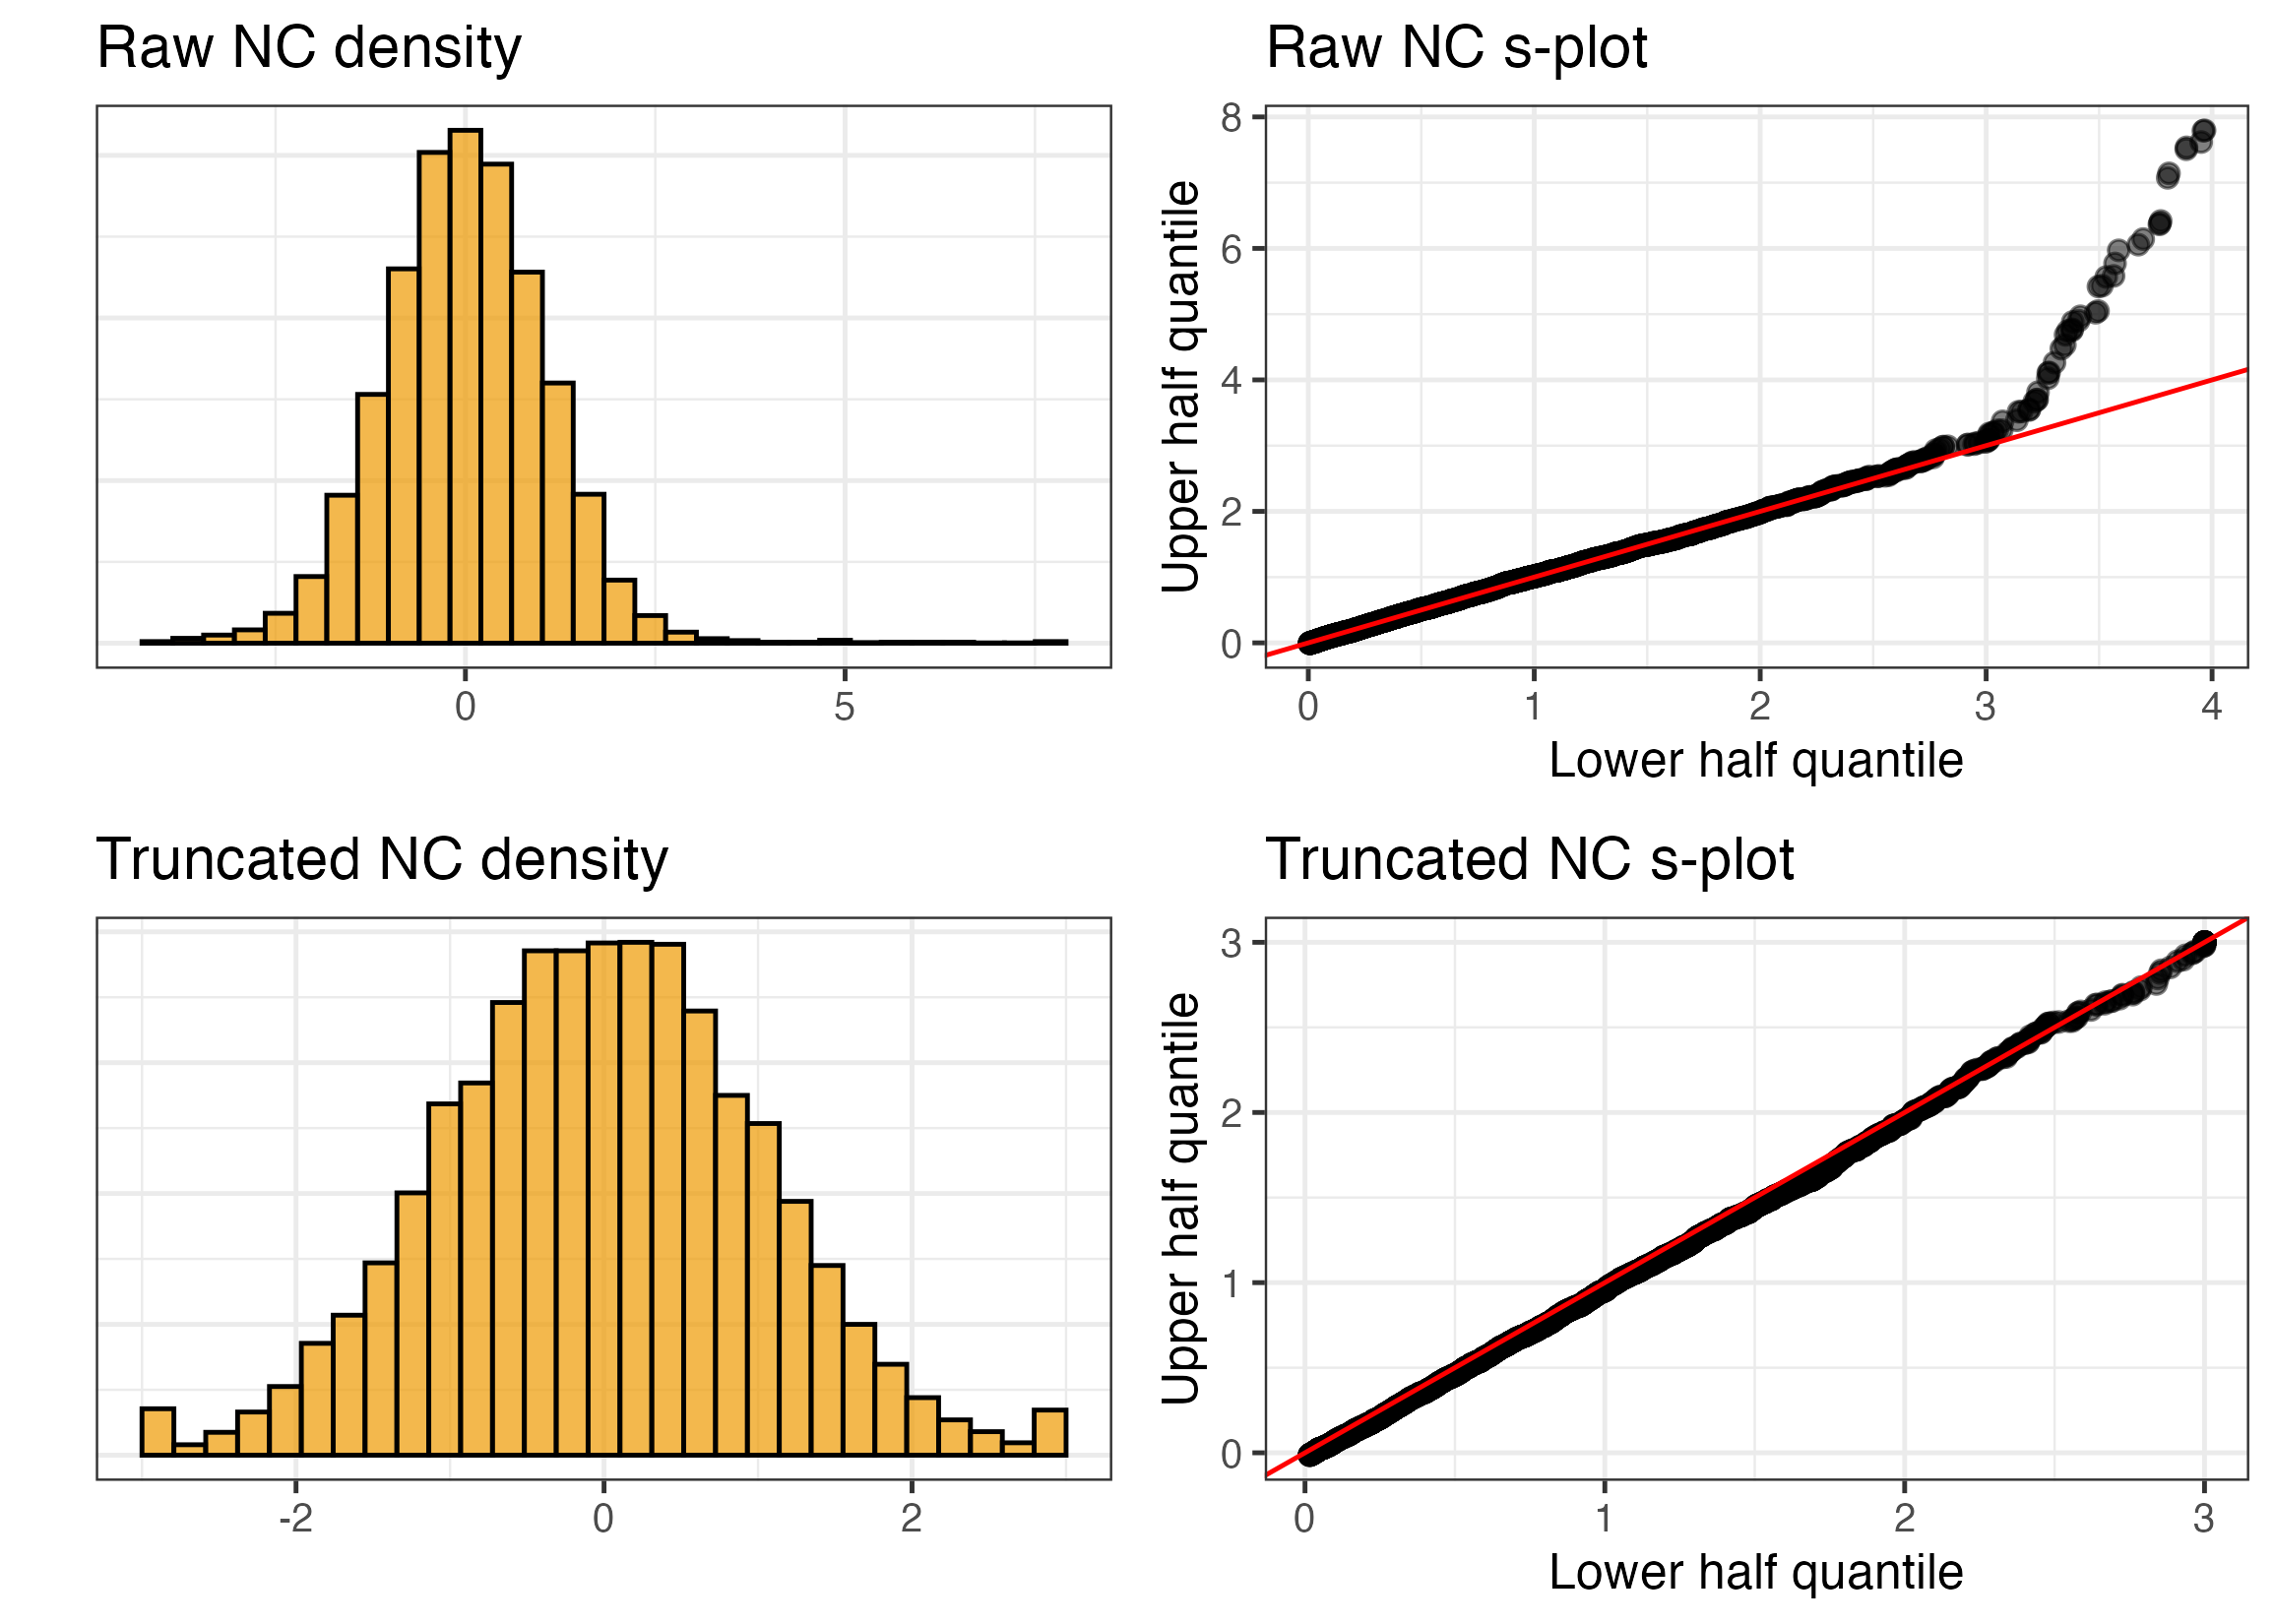
\includegraphics[width=1.0\linewidth]{../figs/bc_robustness_calibration}
	\caption{}
	\label{bcrobustnesscalibration}
\end{figure}


\printbibliography
\end{document}